%!TEX program = xelatex

\documentclass[compress]{beamer}
%--------------------------------------------------------------------------
% Common packages
%--------------------------------------------------------------------------

\definecolor{links}{HTML}{663000}
\hypersetup{colorlinks,linkcolor=,urlcolor=links}

\usepackage[english]{babel}
\usepackage{pgfpages} % required for notes on second screen
\usepackage{graphicx}

\usepackage{multicol}


\usepackage{tabularx,ragged2e}
\usepackage{booktabs}

\setlength{\emergencystretch}{3em}  % prevent overfull lines
\providecommand{\tightlist}{%
  \setlength{\itemsep}{0pt}\setlength{\parskip}{0pt}}


\usetheme{hri}

\usepackage{tikz}
\usetikzlibrary{mindmap,backgrounds,positioning}

\graphicspath{{figs/}}

\title{ROCO318 \newline Mobile and Humanoid Robots}
\subtitle{Part 1 -- Introduction}
\date{}
\author{Séverin Lemaignan}
\institute{Centre for Neural Systems and Robotics\\{\bf Plymouth University}}

\begin{document}

\licenseframe{github.com/severin-lemaignan/module-mobile-and-humanoid-robots}

\maketitle

\imageframe[scale=1]{pepper-robot}
\videoframe[0.56]{figs/NISSAN-ProPILOT-chair.mp4}

\begin{frame}{This module}

    How to build intelligent mobile/humanoid robots?\\
    $\neq$ industrial automation!

    \begin{multicols}{2}

        \begin{center}
            
\includegraphics[height=4.5cm]{no-industrial}

            
\includegraphics[height=4.5cm]{yes-humanoid}
        \end{center}

    \end{multicols}

    \pause

    \begin{itemize}
        \item \textbf{Hardware issues}: sensors, actuators, drive mechanisms, \ldots{}
        \item \textbf{Software issues}: robot control, computer vision, learning robots, \ldots{}
    \end{itemize}

\end{frame}

\begin{frame}{Topics}

\begin{itemize}
\item Sensors for mobile and humanoid robots
\item Computer vision
\item Localisation
\item Robot control
\item Planning and navigation
\item Bipedal robots
\end{itemize}

\end{frame}

\imageframe{industrial-robots-statistics}

\begin{frame}[plain]{}
    But...
\end{frame}

\imageframe{service-robots-stats}



\begin{frame}{Service/domestic robots}


    \begin{multicols}{2}

        \textbf{Service robots}

        \begin{itemize}
            \item
                iRobot Roomba, 12M units sold.
            \item
                Samsung, LG, Dyson
        \end{itemize}
        \vfill
        \columnbreak

        \begin{center}
            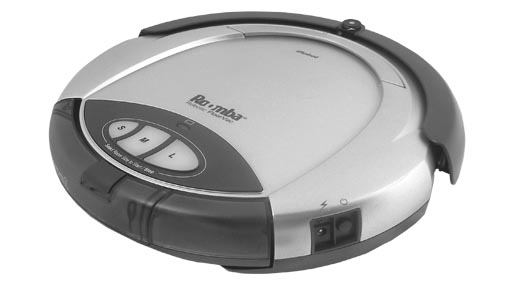
\includegraphics[width=0.5\linewidth]{roomba}
            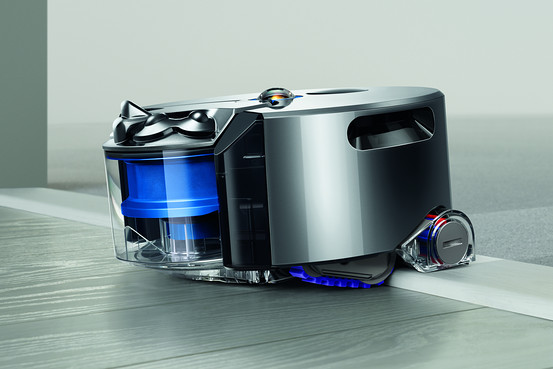
\includegraphics[width=0.5\linewidth]{dyson}
        \end{center}
    \end{multicols}

    \pause

    \begin{multicols}{2}


        \textbf{Edutainment robots}

        \begin{itemize}
            \item \eg KeepOn, 
            \item Lego Mindstorms (original, NXT, EV3),
            \item RoboSapiens
        \end{itemize}
        \vfill
        \columnbreak
        \begin{center}

            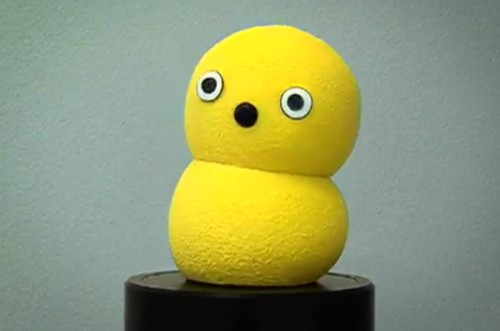
\includegraphics[width=0.6\linewidth]{keepon}

            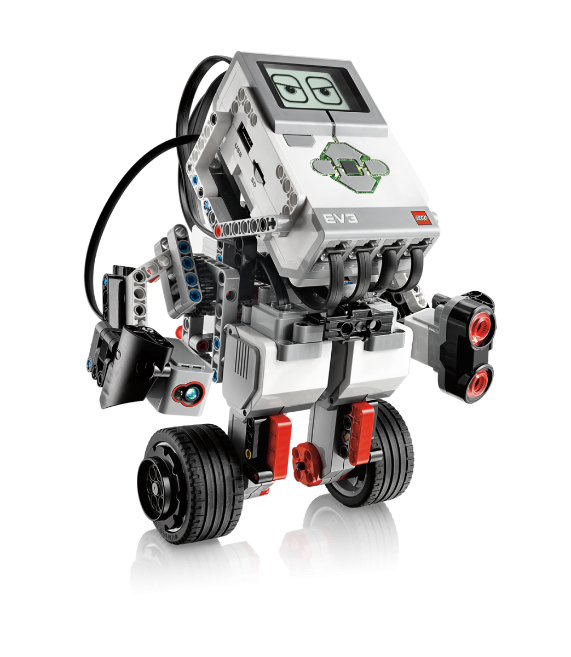
\includegraphics[width=0.5\linewidth]{lego-nxt}
            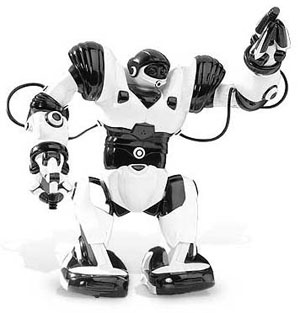
\includegraphics[width=0.5\linewidth]{robosapiens}
        \end{center}
    \end{multicols}
\end{frame}

\begin{frame}{Flying robots}

    \begin{multicols}{2}

Very popular research field and tremendous interest from the military,
some civilian uses (e.g. aerial videoing).

Challenges: autonomy (control of flight parameters), localisation,
energy autonomy, robustness.

    \begin{center}
        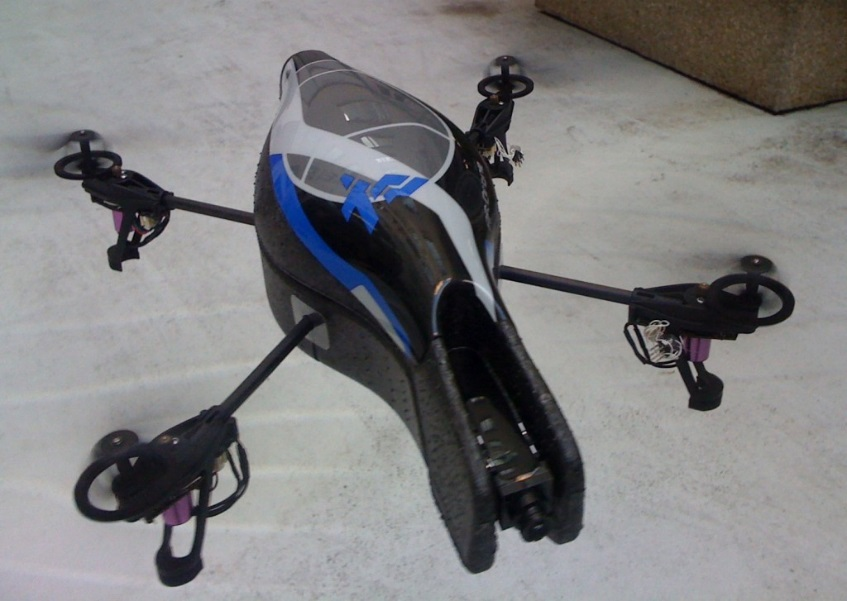
\includegraphics[width=0.8\linewidth]{drone}
    \end{center}

    \end{multicols}
\begin{itemize}
    \item Raffaello D'Andrea's \href{https://www.youtube.com/watch?v=w2itwFJCgFQ}{drone acrobatics}
\item
  \href{http://youtu.be/YQIMGV5vtd4}{U. Pennsylvania, Vijay Kumar's nano
        quadrotors} (see also \href{http://youtu.be/4ErEBkj_3PY}{TED talk})
\item
  EPFL's \href{http://youtu.be/n_qRuHkD5lc}{flying wing robot}.
\end{itemize}

\end{frame}

\begin{frame}{Space exploration}

    \begin{multicols}{2}

        Three Mars rovers:

        \begin{itemize}

            \item
                \href{https://en.wikipedia.org/wiki/Sojourner_(rover)}{Sojourner}
                touched down in summer 1997

            \item \href{http://en.wikipedia.org/wiki/Spirit_rover}{Spirit} and
                \href{http://en.wikipedia.org/wiki/Opportunity_rover}{Opportunity}
                landed in January 2004

            \item \href{http://mars.jpl.nasa.gov/msl/mission/overview/}{Curiosity}
                touched down 5 August 2012

        \end{itemize}

        All are fully teleoperated from earth.  However, the sensors
        and software allow for autonomous obstacle detection and
        navigation.

        Have survived 30x longer than planned;
        \href{http://marsrovers.nasa.gov/}{marsrovers.nasa.gov}

        \begin{center}
            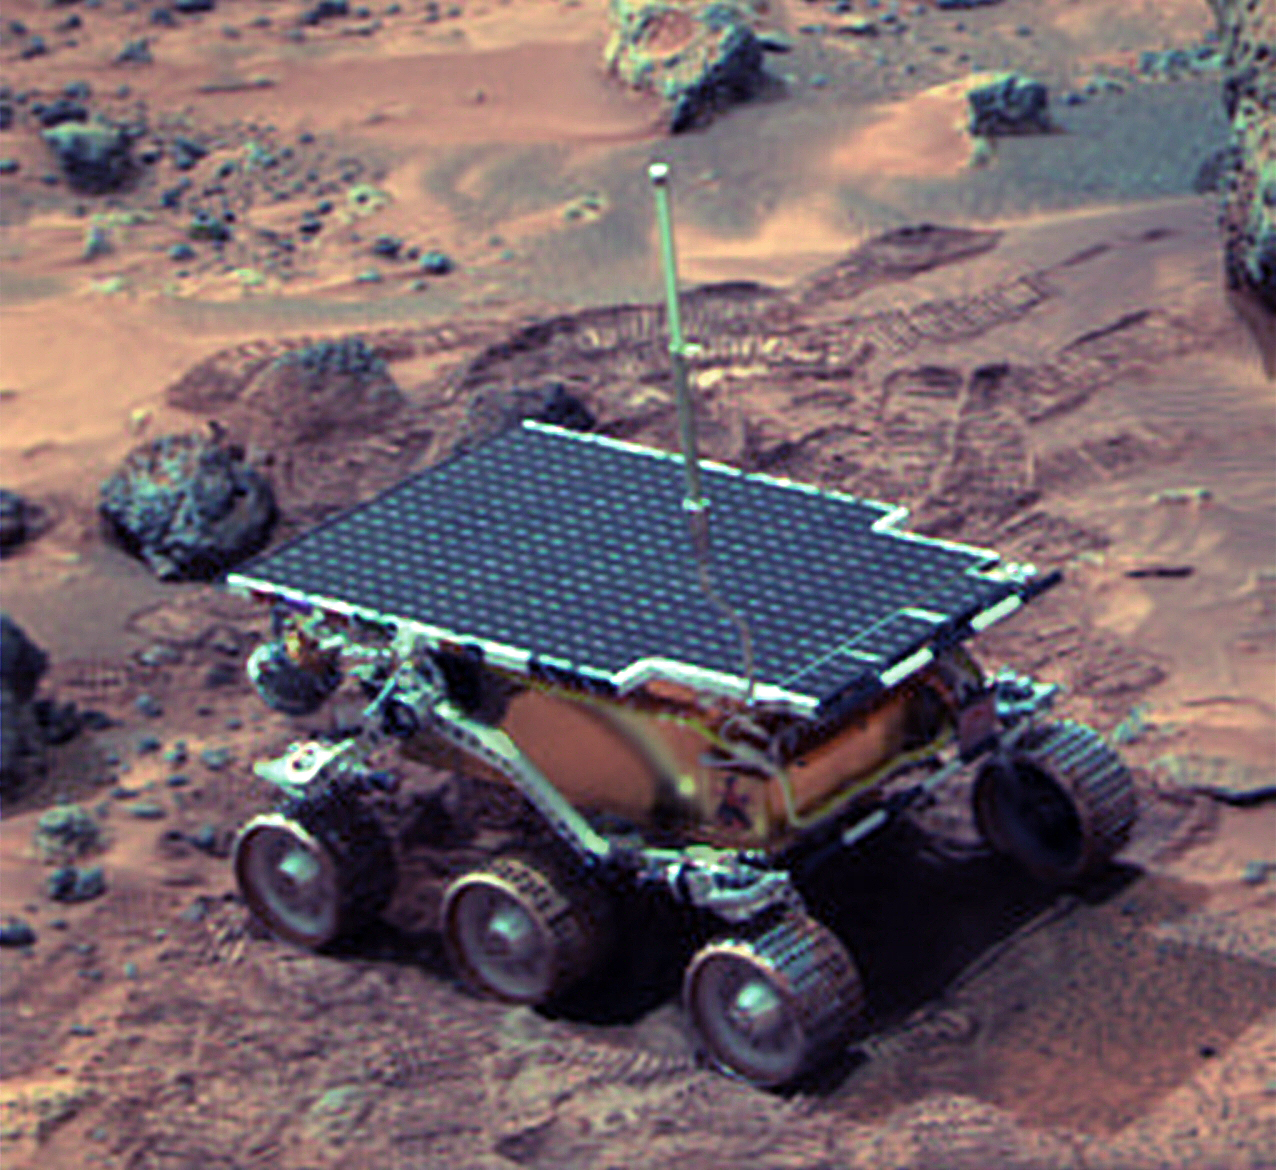
\includegraphics[width=0.6\linewidth]{space-robot-sojourner}

            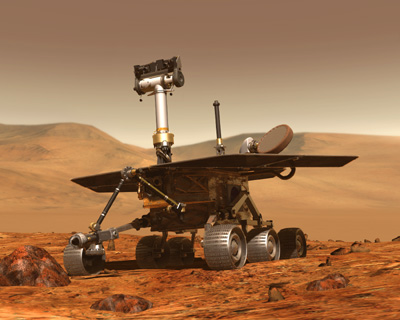
\includegraphics[width=0.6\linewidth]{space-robot-spirit}

            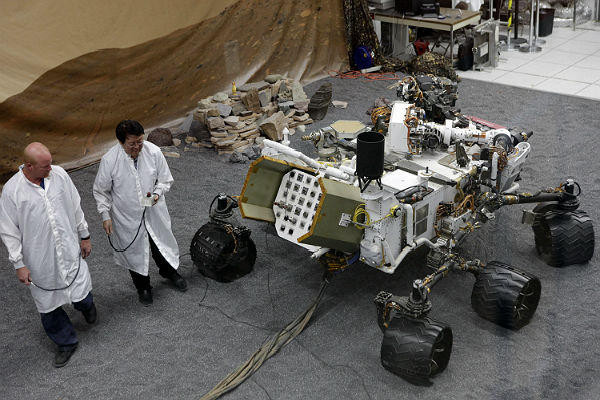
\includegraphics[width=0.6\linewidth]{space-robot-curiosity}
        \end{center}
    \end{multicols}
\end{frame}

\begin{frame}{Defence robots}

Best selling ``professional service'' robot: 6500 units in 2011, 6100 in
2012, 9500 in 2013.

\begin{itemize}
\item
  ``This robot has no fear''.
\end{itemize}

See IEEE Spectrum
\href{http://spectrum.ieee.org/robotics/military-robots/autonomous-robots-in-the-fog-of-war/0}{Autonomous
Robots in the Fog of War}

Videos

\begin{itemize}
\item
  \href{http://youtu.be/eaP0waiz43w}{iRobot packbot}
\end{itemize}

\end{frame}

\begin{frame}{Autonomous cars}

Self-driving cars

From a \textgreater{}200km race for autonomous ground vehicles across
the Mojave/Nevada desert (DARPA grand challenge) to the
Google/BMW/Mercedes/Audi/\ldots{} car.

Video

\begin{itemize}
\item
  \href{http://youtu.be/M2AcMnfzpNg}{Overview of 2nd DARPA Grand
  Challenge 2005}
\item
  \href{http://youtu.be/cdgQpa1pUUE}{Google Car promo video}
\end{itemize}

\end{frame}

\begin{frame}{Humanoids}

Human-like robots.

Tremendously challenging

\begin{itemize}
\item
  Power, actuations, artificial intelligence, perception, control,
  walking, \ldots{}
\end{itemize}

Videos

\begin{itemize}
\item
  \href{http://youtu.be/yND4k4NM0qU}{Honda Asimo latest version}
\item
  \href{http://youtu.be/aqCmX5dMYHg}{Boston Dynamics Petman prototype}
  and \href{http://youtu.be/FFGfq0pRczY}{obstacle negotiation}.
\item
  \href{https://www.youtube.com/watch?v=g0TaYhjpOfo}{DARPA Robotics
  challenge 2015 outtakes}
\end{itemize}

\end{frame}

\begin{frame}{And what do I do?}

Cognitive robotics

\begin{itemize}
\item
  Building robots and their artificial intelligence inspired on natural
  systems, such as developing children
\end{itemize}

Human-Robot Interaction

\begin{itemize}
\item
  Building robots that can work alongside people, using social cues that
  people use to communicate
\item
  \href{http://tedxtalks.ted.com/video/The-power-of-robots-with-a-face}{TEDxTalk}
\end{itemize}

\end{frame}


\begin{frame}{}
    \begin{center}
        \Large
        That's all, folk!\\[2em]
        \normalsize
        Questions:\\
        Portland Square A216 or \url{severin.lemaignan@plymouth.ac.uk} \\[1em]

        Slides:\\ \url{github.com/severin-lemaignan/[REPO]}

    \end{center}
\end{frame}



\end{document}
